% Para documento texto corto
\documentclass[paper=letter,oneside,fontsize=12pt, parskip=full]{article}
%\documentclass[paper=letter,oneside,fontsize=11pt, parskip=full]{scrartcl}
%\documentclass{amsart}
%\documentclass[paper=letter,oneside,fontsize=12pt]{scrartcl}

% Establece dimensiones de los margenes
% \usepackage[inner=1.5cm,outer=3cm,top=2cm,bottom=4cm,
% bindingoffset=5mm]{geometry}
\usepackage[left=3cm,right=3cm,top=3cm,bottom=3cm,
bindingoffset=0cm, footskip=0.5cm, headheight=2cm]{geometry}

% Elimina sangrias y aumenta espacio entre parrafos
\usepackage{parskip}

% Permite cambiar margenes derecho e izquierdo
% de secciones de texto con el entorno
% adjustwidth
\usepackage{changepage}

% Permite establecer el espaciado entre lineas
\usepackage{setspace}

% Permite ingresar caracteres acentuados y especiales 
% sin necesidad de emplear comando
% utf8 codificacion de entrada Unicode (mas simbolos que ASCII)
\usepackage[utf8]{inputenc}

% Formato direccione URL
% \usepackage{hyperref}

% T1 encoding for European, English, American text
\usepackage[T1]{fontenc}
% Fuente escalable
\usepackage{lmodern}

% Reemplazo para fuente Arial
% \usepackage{helvet}
% Usa la fuente sans-serif por defecto
% \renewcommand{\familydefault}{\sfdefault}

% Carga babel, idioma ingles
\usepackage[english, spanish]{babel}

% Mejor jsutificacion, tipografia alta calidad.
\usepackage{microtype}
% Para unir columnas y filas en tablas
\usepackage{array}

% Agrega comandos extra al comando tabular
% \toprule, \midrule, \bottomrule
\usepackage{booktabs}
% Tablas con ancho establecido por usuario
\usepackage{tabularx}
% Para posicionamiento preciso de tablas dentro del texto

% Tabla de tres secciones
\usepackage[flushleft]{threeparttable}

\usepackage{float}

% Unir filas en tablas
\usepackage{multirow}

% Permite controlar colores de tablas
\usepackage{xcolor, colortbl}

% Encabezados personalizados
\usepackage{fancyhdr}
\usepackage{graphicx}

% Permite obtener el numero de la ultima pagina
\usepackage{lastpage}

% Paquetes para figuras
% Paquete caption para titulos figuras
% Paquete subcaption para subfiguras
\usepackage{caption}
\usepackage{subcaption}

% Espaciado inteligente
\usepackage{xspace} 

% Para formato de codigo fuente
\usepackage{xcolor}
\usepackage{listings}
% Etiquetas de listandos codigo en españo

% Para diagramas de bloques entre otros
\usepackage{smartdiagram}

\renewcommand\lstlistingname{Listado}

\lstset{basicstyle=\ttfamily,
	showstringspaces=false,
	commentstyle=\color{red},
	keywordstyle=\color{blue}}

% Definicion de tipos de columnas tabla
\newcolumntype{C}[1]{>{\centering}m{#1}}
\newcolumntype{L}[1]{>{\raggedleft}m{#1}}
\newcolumntype{R}[1]{>{\raggedright}m{#1}}

% Cabeceras
\pagestyle{fancy}
% Borra cabecera y pie actuales
\fancyhead{}
% Cintillo cabecera
%\chead{
%	\includegraphics[width=150mm]{Imagenes/Cabecera.png}
%}
%\fancyhead[L]{\includegraphics[width=0.3\textwidth]{Imagenes/cabecera.pdf}}
%\fancyfoot[C]{ 
%	\begin{tabularx}{\textwidth}{|m{2.0cm}|X|m{2.5cm}|m{2.0cm}|}
%		\hline			
%			\centering
%			\includegraphics[height=0.8cm]{Imagenes/pie-izq.pdf} &			
%			\centering
%			Confidencial &
%			\centering
%			\includegraphics[height=0.8cm]{Imagenes/pie-der.pdf}  &			
%			\thepage~/~\pageref{LastPage} \\
%		\hline 
%	\end{tabularx}	 
%}

% Comando para formatear y justificar parrafos de código y 
% comandos de shell
% \newcommand{\code}[1]{
%	\begin{adjustwidth}{1.5cm}{0.0cm}
%		\ttfamily
%		#1
%	\end{adjustwidth}}	

% Entorno para formato de secciones de codigo
\newenvironment{code}
	{\begin{adjustwidth}{1.5cm}{0.0cm}\ttfamily}
	{\end{adjustwidth}}

% Entorno para formato de secciones de enlaces
\newenvironment{link}
	{\ttfamily}{}	
	
\definecolor{colorfa}{rgb}{0.3569,0.608,0.8353}
\definecolor{colorfb}{rgb}{0.4392,0.678,0.2784}
\definecolor{colorfc}{rgb}{1.0000,0.361,0.0000}
\definecolor{colorsem}{rgb}{0.1804,0.455,0.7098}
\definecolor{colorfd}{rgb}{0.9294,0.490,0.1922}
\definecolor{colorfe}{rgb}{0.2667,0.329,0.4157}

\newcommand{\fa}{\cellcolor{colorfa}}
\newcommand{\fb}{\cellcolor{colorfb}}
\newcommand{\fc}{\cellcolor{colorfc}}
\newcommand{\sem}{\cellcolor{colorsem}}
\newcommand{\fd}{\cellcolor{colorfd}}
\newcommand{\fe}{\cellcolor{colorfe}}

% Numeracion de paginas
% numeros arabigos
\pagenumbering{arabic}

	\begin{document}
		
		%\title{Informe de Avance de Pasantía}
		%\author{Jose Arias}
		%\address{correo@josearias.com.ve}
		%\date{Septiembre, 2017}
		
		%\maketitle
			
		\begin{titlepage}
		
		\begin{center}		
			
			%\vspace{10cm}
			% 12 puntos = fuente large
			\begin{large}							
				\bfseries
				\uppercase{Universidad Central de Venezuela} \\			
				\uppercase{Facultad de Ingeniería} \\							
				\uppercase{Escuela de Ingeniería Eléctrica} \\
        		\uppercase{Departamento de Electrónica, Computación y Control} \\
        		\uppercase{Informe de Avance de Pasantía}          	
			\end{large}			
		
			\vfill
			
			\begin{large}
				\bfseries
				\uppercase{Informe de Avance de Pasantía}
			\end{large}
		
			\vspace{2mm}
			
			% 16 puntos = fuente Large de 14 puntos			
			\begin{Large}
				\begin{spacing}{1.2}
					\bfseries				
		      		\uppercase{Diseño de un equipo electrónico controlador de interruptores y atenuadores empleado en la medición de la figura de ruido en dispositivos de radio frecuencia}	
		      	\end{spacing}
			\end{Large}					
			
			\vfill
			
			\begin{flushright}
				Br. Arias Bustamante, Jose A. \\
				C.I. 14.66.744.
			\end{flushright}
		
			\vfill
			
			\begin{center}
				Caracas, septiembre 2017.
			\end{center}
		
		\end{center}
	
	\end{titlepage}
	
	\clearpage
	
	\tableofcontents
		
	\section{Introducción}
		Describe el proceso de instalación adaptador USB/GPIB Agilent 82357B, la instalación y construcción de la librería c de soporte (\texttt{linux-gpib}) a partir del código fuente y la obtención y carga del firmware para el adaptador.
		
	\section{Descripción del Proyecto}
	
	En la figura \ref{Fig:SistemaMedicionFiguraRuido} se muestra un sistema propuesto por Agilent Technologies para medición de la figura de ruido en dispositivos de radio frecuencia y de microondas. Este sistema esta conformado por tres instrumentos fundamentales.
	
	\begin{figure}[!h]
		\begin{center}
			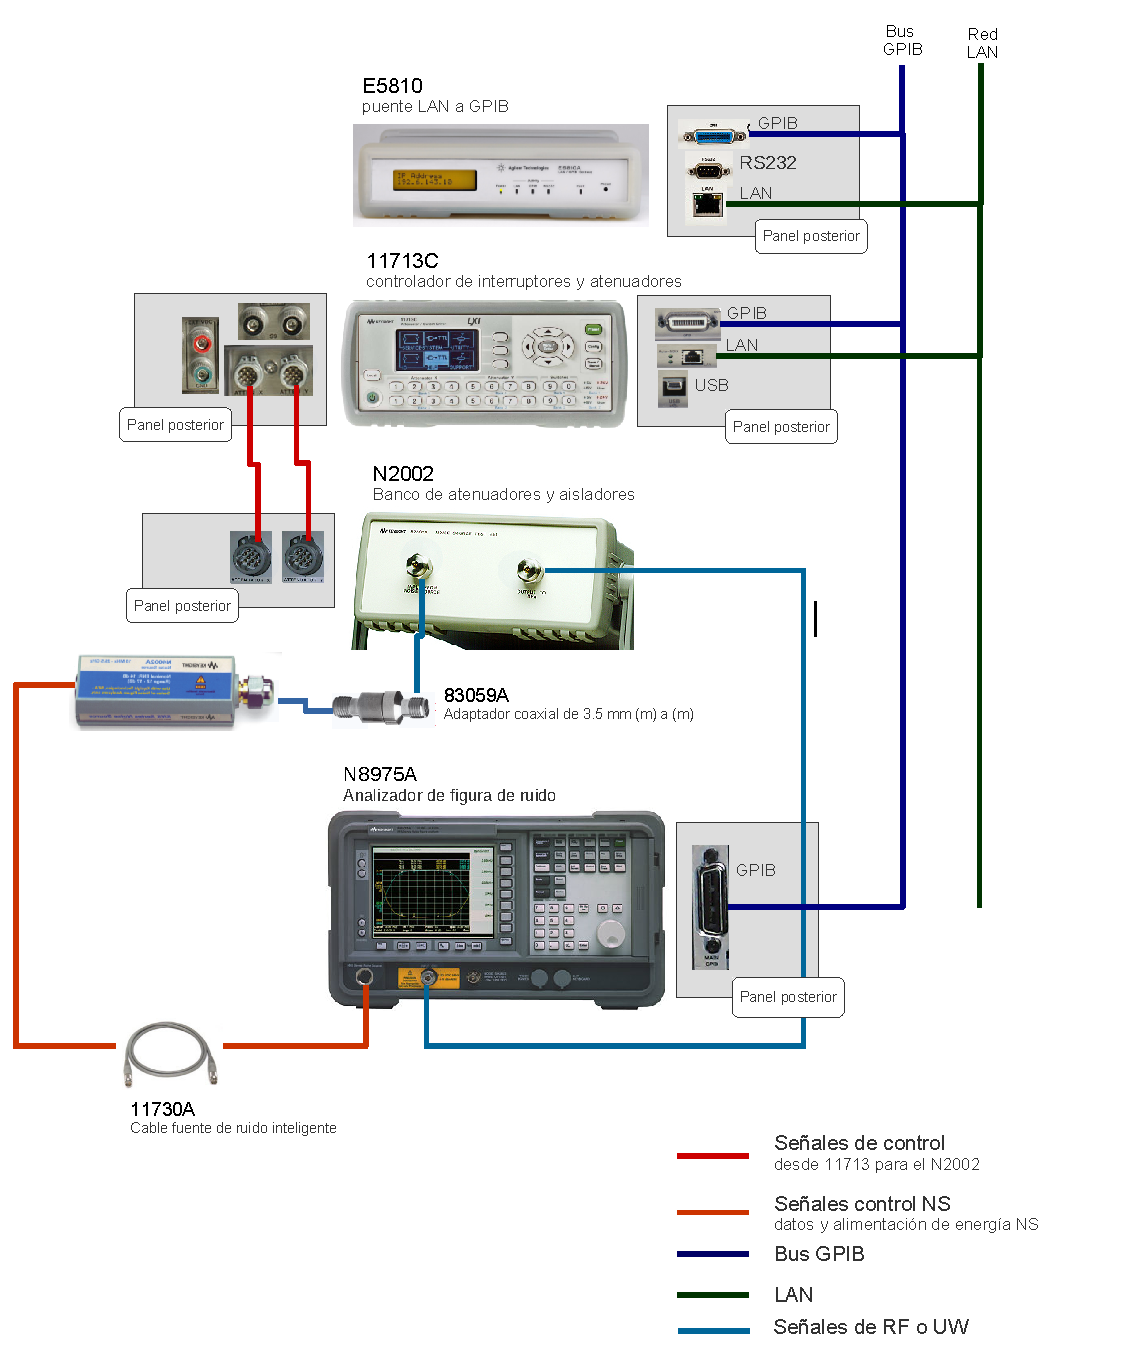
\includegraphics[height=6cm]{Imagenes/SistemaMedicionFiguraRuido.pdf}
			\caption{Sistema para medición de figura de ruido}
			\label{Fig:SistemaMedicionFiguraRuido}
		\end{center}	
	\end{figure}	
	
	\begin{table}[h!]
		\begin{tabular}{p{3cm}l}
			\begin{minipage}{3cm}
				\includegraphics[width=3cm]{Imagenes/N8975A.pdf}
			\end{minipage} &
			Analizador de figura de ruido (NFA) N8975A \\

			\begin{minipage}{3cm}
				\includegraphics[width=3cm]{Imagenes/N2002A.pdf}
			\end{minipage} &
			Equipo para pruebas con fuente de ruido N2002A \\
			
			\begin{minipage}{3cm}
				\includegraphics[width=3cm]{Imagenes/11713A.pdf}
			\end{minipage} &			
			Controlador electrónico de interruptores y atenuadores, serie 11713 
		\end{tabular}
	\end{table}

	De los tres equipos listados, el Cendit dispone solo dos de ellos: el analizador de figura de ruido N8975A y el equipo para pruebas con fuente de ruido N2002A. Para que la institución pueda colocar en servicio el SMFR, requiere del controlador electrónico de atenuadores de la serie 11713 de Keysight Technologies. Por motivos presupuestarios, este equipo no ha podido ser adquirido.
	
	Para suplir esta carencia, el Cendit requiere el diseño de un equipo electrónico que pueda suplir la funcionalidad de los equipos de la serie 11713 dentro del sistema. El diseño de este dispositivo es el tema del TEG del cual este documento es un informe de avance de pasantía.
	
	\begin{figure}[!h]
		\begin{center}
			\includegraphics[width=17cm]{Imagenes/DiagramaBloquesSistema.pdf}
			\caption{Esquema de sistema para medición de figura de ruido}
			\label{Fig:SistemaMediciónFiguraRuido}
		\end{center}
	\end{figure}		


	\subsection{Metodología de trabajo}
	
	\subsection{Metodología inicial}
	
	Al iniciar la pasantía en el Cendit, en el anteproyecto de TEG entregado como parte de los recaudos exigido para su inscripción, se planteo el cronograma de actividades a seguir durante el desarrollo del proyecto que se muestra en la tabla \ref{Tab:CronogramaActividadesInicial}.
	
	\begin{threeparttable}[!h]
		\centering
		\arrayrulecolor{gray}
		\setlength{\extrarowheight}{4pt}		
		\resizebox{\textwidth}{!}{
		\begin{tabular}{|c|l|l|l|l|l|l|l|l|l|l|l|l|l|l|l|l|l|l|l|l|l|l|l|l|l|l|l|l|}
			\hline 			
			\textbf{Semanas} & 1 & 2 & 3 & 4 & 5 & 6 & 7 & 8 & 9 & 10 & 11 & 12 & 13 & 14 & 15 & 16 & 17 & 18 & 19 & 20 & 21 & 22 & 23 & 24 & 25 & 26 & 27 & 28 \\
			\hline
			\textbf{Fase 1}
			& \fa & \fa & \fa & \fa & \fa & \fa & & & & & & & & & & & & & & & & & & & & & & \\			
			\hline			
			\textbf{Fase 2} & & & & & & & \fb & \fb & \fb & \fb & \fb & \fb & \fb & \fb & \fb & \fb & \fb & & & & & & & & & & & \\
			\hline
			\textbf{Fase 3} & & & & & & & & & & & & & & & & & & \fc & \fc & \fc & \fc & \fc & & & & & & \\	
			\hline		
			\textbf{Seminario} & & & & & & & & & & & & & & \sem & & & & & & & & & & & & & & \\
			\hline
			\textbf{Fase 4} & & & & & & & & & & & & & & & & & & & & & & & \fd & \fd & \fd & \fd &  & \\
			\hline
			\textbf{Fase 5} & & & & & & & & & & & & & & & & & & & & & & & & & & & \fe & \fe \\
			\hline	
		\end{tabular}
		}
		\begin{tablenotes}
			\item Fecha de inicio: 6 de Marzo de 2017. 
			\item Jornada de 8 horas diarias, lunes a viernes, de 8:00 AM a 12:00 M y de 1:30 PM a 4:30 PM.
		\end{tablenotes}
		\caption{Cronograma de actividades inicial}			
		\label{Tab:CronogramaActividadesInicial}
	\end{threeparttable}
	
	La ejecución de proyecto se dividió en cinco fases, a desarrollar en un lapso de 28 semanas. A continuación se da una descripción general de las actividades propuestas en cada fase.

	\begin{table}[!h]
		\begin{tabular}{rp{13cm}}
			\textbf{Fase 1} & Preparación e investigación. Dedicada a investigar el funcionamiento de cada uno de los equipos que integran el sistema de medición de figura de ruido. La recopilación y lectura de la documentación de estos equipos que ofrecen las empresas Agilent y Keysight y a través de ensayos sobre el sistema se obtendrá un entendimiento del funcionamiento del mismo. La información obtenida se plasmará en un informe descriptivo del SMFR. \\			
			\textbf{Fase 2} & Diseño de hardware. Comienza con la formulación de un concepto para un equipo que permita suplir la funcionalidad de un equipo de la serie Keysight 11713. Por medio de un proceso iterativo que implica el diseño de hardware, de firmware y mecánico se logrará la documentación de diseño, que permita construir el hardware en la siguiente fase.	\\		
			\textbf{Fase 3} & Implementación del hardware. Se construirá el hardware diseñado y se verificará su desempeño dentro del SMFR. Esta fase implica la depuración firmware y software además de verificar que el hardware cumpla los objetivos de diseño. \\
			\textbf{Fase 4} & Preparación de manuales. Se producirá un manual de usuario para el equipo implementado, que contendrá instrucciones para instalación, operación y resolución de fallas. \\
			\textbf{Fase 5} & Preparación de documentos Cierra el proyecto con la preparación de un informe de pasantía para el Cendit. También se elabora el tomo parra TEG, a presentar en la Escuela de Ingeniería Eléctrica de la UCV.
		\end{tabular}
	\end{table}

	Diversos contratiempos surgidos en los últimos meses han impedido completar algunas de las fases en el tiempo estipulado, provocando que la fases anteriores se traslapen que le prosiguen.
	
	La situación de conflictividad que se presento en la ciudad de Caracas en los últimos meses provocó que el Cendit se viese obligado a recortar la jornada laboral e incluso suspender días completos de actividad en varias ocasiones, para resguardar la integridad física del personal.
	
	Se debe considerar que el proyecto asignado presenta un buen grado de complejidad, 
	abarca el diseño y desarrollo de hardware, software y firmware. En un proyecto complejo, resulta difícil especificar de antemano un plan de trabajo, que detalle con exactitud las actividades a realizar y su extensión en tiempo, antes de involucrarse de lleno en su desarrollo. 
	
	En vista de lo anterior, en este tipo de proyectos, se debe considerar que el cronograma planteado es tentativo, no ha podido ser seguido al pie de la letra, sin embargo ha servido como una guía de la secuencia general de actividades a realizar.

	Las actividades de investigación y desarrollo realizadas para la ejecución del TEG hasta la fecha, han demostrado que el proyecto requiere de tiempo adicional.	

	\section{Actividades Realizadas}
	
	En esta sección se detallan de forma sucinta las actividades realizadas en el desarrollo del TEG, para cada una de las fases, en los últimos 5 meses.
	
	\subsection{Documentación}
	
	Correspondientes a la  fase 1, las tareas de documentación realizadas son las siguientes
	
	\begin{itemize}
		\item Investigación sobre caracterización de dispositivos en alta frecuencia: parámetros de dispersión.
		\item Investigación sobre edición de figura de ruido en RF y microondas.
		\item Documentación acerca de cada uno de los instrumentos que integran el SMFR.
		\item Documentación acerca del software asociado o que brinda soporte al SMFR.				
	\end{itemize}	
	
	Para entender con propiedad el funcionamiento del SMFR, se debe entender el concepto de figura de ruido. Se realizó un estudio sobre la medición de figura de ruido en dispositivos de RF y microondas, haciendo énfasis en la técnica de medición de figura de ruido conocida como el método del factor Y, la cual es empleada por el SMFR.
	
	Como el sistema mide figura de ruido en dispositivos de alta frecuencia, fue necesario estudiar el concepto de parámetros de dispersión en dispositivos de RF y de microondas. Los parámetros de dispersión son utilizados para caracterizar en frecuencia a dispositivos multipuertos en alta frecuencia, de forma análoga a las matrices de impedancia o admitancia.
	
	Se recopiló la documentación asociada a los instrumentos y componentes que integran el SMFR. Esta documentación, en forma de manuales de usuario, notas técnicas y hojas de datos, se consiguió de forma libre en internet, en los sitios web de Keysight Technologies y Agilent Technologies. 	
	
	\subsection{Investigación y recopilación de software asociado al SMFR}
	
	El proceso de medición en el SMFR puede ser totalmente automatizado por medio de aplicaciones de software apropiadas. El estudio de la documentación del SFMR permitió conocer que existe un buen soporte de software para este sistema, en forma de librerías, entornos de desarrollo y programas de utilidad general.
	
	El estudio de la documentación permitió conocer que existe una especificación que estandariza las comunicaciones entre instrumentos a través de diversos medios de transporte de datos en instrumentos de prueba y medición (Test \& Measurement), como  el bus de interfaz de propósito general (GPIB), o sobre protocolos como TCP/IP o USBTMC empleando puertos estandarizados de PC. Esta especificación se conoce como Virtual Instrument Software Architecture, conocida comúnmente como VISA, es una API que brinda una interfaz uniforme al programador para las operaciones de intercambio de datos. 
	
	Keysight Technologies suministra un amplio soporte de software para los dispositivos del SFMR, en especial un paquete de software conocido como Keysight IO Libraries Suite, que contiene las librerías VISA, exclusivamente para ambiente Windows. 
	
	National Instruments también proporciona librerias VISA para ambiente Windows y para algunas distribuciones de Linux, entre las cuales no se encuentra Ubuntu, 
	sistema operativo que se empleado en el Cendit.
	
	Se realizo un estudio y pruebas con las aplicaciones contenidas en la suite de Keysight, y se empleo la librería VISA que contiene para acceder a los instrumentos del SMFR en ambiente Windows.
	
	Como el Cendit requiere el uso de software libre, se intento instalar las librerías VISA que National Instruments ofrece para Linux, sin resultados satisfactorios, ya que esta empresa proporciona una librería para Ubuntu.	
	
	Ante la carencia de una librería VISA que pueda ejecutarse en Ubuntu, se buscaron alternativas, por ejemplo para el acceso a instrumentos en el bus GPIB se logró por medio de la librería conocida como linux-gpib.
	
	\subsection{Investigación e instalación de aplicaciones de software}
	
	Para la elaboración de documentos se instalo el paquete de oficina \emph{LibreOffice} en su versión 5.3.4.2.
	
	Para generar documentos con formato pdf con alta calidad tipográfica, se instaló una distribución de \LaTeX conocida como \emph{TeX Live} (https://www.tug.org/texlive/) acorde al sistema operativo Ubuntu. 
	
	Obtenida esta distribución de \LaTeX, fue necesario instalar un editor de documentos en formato .tex conocido como \emph{TeX Studio} (http://texstudio.sourceforge.net/). 
	
	Los cálculos matemáticos se realizaran por medio de dos herramientas de software: un paquete de calculo simbólico y una aplicación para cálculo númerico. Para el cálculo simbólico se emplea \emph{Maple} version 13 para Linux y para el cálculo matricial se emplea el software de fuente libre \emph{Scilab} (https://www.scilab.org/) versión 6.0.0
	
	El desarrollo tanto de software como de firmware existen aplicaciones de software que facilitan en gran medida en trabajo del desarrollador, conocidas como \emph{entornos de desarrollo integrados}, \emph{IDE} por sus siglas en ingles. Las herramientas IDE permitan gestionar cada una de las actividades implicadas durante el ciclo de vida de desarrollo: edición de código, compilación,  depuración, administración de dependencias y librerías y control de versiones.
	
	Para el desarrollo de firmware con microcontroladores y dispositivos de Microchip, se emplea el MPLAB IDE, versión 3.50 para Ubuntu.
	
	Para el desarrollo de aplicaciones de escritorio en C/C++ se instaló la \emph{plataforma de desarrollo de software} conocida como \emph{QT} (https://www1.qt.io/es/). El interés por usar esta herraienta es que incluye un SDK - Source Development Kit, el cual es un conjunto de librerías que da soporte al diseño de interfaces gráficas y, además, integra un IDE conocido como QT creator.
	
	El desarrollo de aplicaciones Java requiere el uso de una distribución del JDK -Java Development Kit- apropiado para sistema operativo Linux. Se emplean dos variantes de JDK, con fines de establecer diferencias. Se instalaron la distribución del JDK de Oracle (http://www.oracle.com/technetwork/es/java/index.html) en  su versión 1.8.0 y la implementación en código abierto  suministrada por OpenJDK (http://openjdk.java.net/) con versión 1.7.0.
	
	El IDE empleado para el desarrollo de aplicaciones Java es \emph{Intelli J IDEA} (https://www.jetbrains.com/idea/).
	
	Como se hace uso del \emph{lenguaje unificado de modelado}, UML por sus siglas en ingles, para el diseño de software, se instaló una aplicación que permita generar los distintos tipos de diagramas UML. La aplicación elegida para este fin es \emph{StarUML} (http://staruml.io/), version 2.8.0.
	
	\subsection{Desarrollo de software}
	
	Para el desarrollo de software se comenzó elaborando el concepto de la aplicación dentro del SMR que se muestra el la figura 
	
	\begin{figure}[!h]
		\begin{center}
			\includegraphics[width=18cm]{Imagenes/SystemMainDiagram.pdf}
			\caption{Diagrama de Bloques Hardware}
			\label{Fig:Diagrama de Bloques de Hardware}
		\end{center}
	\end{figure}		
	

	\subsection{Investigación de librerías de software}
	
	La aplicación CenditLab presentará una interfaz gráfica, se decide emplear \emph{JavaFX} la cual es una tecnología dentro del ecosistema Java que permite desarrollar \emph{aplicaciones de internet enriquecidas} (rich internet application - RIA). De esta tecnología se toma la facilidad que brinda para desarrollar interfaces de usuario de alta calidad.
	
	CenditLab otorgará al usuario la funcionalidad de generar reportes de resultados en formato pdf. Para ello se estudio la librería \emph{iText} (https://sourceforge.net/projects/itext/) de Java, la cual perite al programador crear y manipular documentos pdf a través de código.	
	
	\subsection{Informe técnico descriptivo del SMFR}	
	
	\subsection{Diseño de software}
	
	\subsection{Ingeniería de software}	
	
	\subsubsection{Captura de requerimientos}
	
	Para sistema de medición de ruido de la figura \ref{Fig:SistemaMedicionFiguraRuido} se diseñará e implementará una aplicación de software que permita gestionar y automatizar el proceso de medición con el SMFR empleando un PC. Conocidas como aplicaciones para sistemas \emph{Test and Measurement (T \& M)}, Keysight Technologies suministra varias aplicaciones de este tipo, para ambiente Windows, su uso requiere de la compra de una licencia, aunque se pueden descargar versiones pruebas con limite de tiempo. El Cendit requiere que el desarrollo de la aplicación se haga bajo los principios que rigen el software libre, destinada inicialmente a ejecutarse en Ubuntu.	
	
	Se inicio la captura de requerimientos de software por medio de dos vías: el estudio de aplicaciones de tipo T \& M y captura de requerimientos por parte de los usuarios potenciales dentro del Cendit. En la primera de ellas se estudiaron las características esenciales del software para ambiente Windows que suministra la empresa Keysight Technologies, entre estas se tienen aplicaciones como BenchVue o Keysight VEE Pro la cual es un entorno de programación de instrumentos gráfico, que  guarda buena similitud con la aplicación de National Instruments LabView. 	
	
	Se estudiaron además las aplicaciones de tipo T \& M que dispone el Cendit, entre ellas la aplicación conocida como \emph{EmcTest32} en el laboratorio de compatibilidad electromagnética conducida (EMC), empleada para el control de la instrumentación que se emplea en ensayos de EMC en equipo electrónico.
	
	El estudio se enfoco en dos aspectos fundamentales de estas aplicaciones, como lo son la interfaz de usuario y sus funciones principales. 
	
	Dentro del Cendit, su personal técnico cuenta con amplia experiencia en el uso de aplicaciones de tipo T \& M, en especial para ensayos de EMC por medios guiados y radiados. Es por ello que se considero la opinión de la Ing. Katherine Moncada y el TSU José Rodriguez sobre la funcionalidad que debe brindar una aplicación que autoatice el proceso de medición de figura de ruido.  También resulto de importancia la opinión que dieron los usuarios potenciales de la futura aplicación dentro del Cendit, ya que ellos cuentan con la experiencia en el uso de estas aplicaciones. Se seleccionaron dos miembros del personal Cendit dieron sus 	
	
	Para sistematizar el proceso de captura de requerimientos de software, el tutor sugirió estudiar los estándares ISO/IEC/IEEE, que brindan un marco teórico y una metodología estandarizada para la captura de requerimientos de sistemas de software. Los documentos estudiados se lista a continuación,
	
	\begin{enumerate}  
		\item Systems and Software Engineering Architecture Description (ISO/IEC/IEEE 42010, 2011).		
		\item System and Software Engineering Life Cycle Processes Requirements Engineerng (ISO/IEC/IEEE 29148, 2011).
		\item Systems and Software Engineering Vocabulary (ISO/IEC/IEEE 24765, 2011).	
	\end{enumerate}
	
	El documento número 1 brinda una base conceptual, en el se definen de cada uno de los elementos e integrantes involucrados en desarrollo de un sistema de software. A partir de la definición de las partes, detalla como se interrelacionan entre si para formar lo que en el documento se conoce como la arquitectura del sistema. 
	
	Del documento número 2 se obtienen pautas para elaborar el documento de captura de requerimientos de software. Este documento trata sobre la ingeniería de requerimientos, definida como una disciplina interdisciplinaria que se encarga de mediar entre los dominio de las personas participantes del sistema para así establecer los requisitos que este debe cumplir. De este documento se obtienen las características que debe poseer un sistema de software bien plateado, además del esquema del documento escrito que los contiene.
	
	El documento 3 es un glosario que contiene la definición de una gran cantidad de términos de uso común en la ingeniería de software. Pretende estandarizar la terminología.	
	
	\subsubsection{Documento de captura de requerimientos de software}
	
	Con la información obtenida en la sección anterior, se procede a elaborar el documento de requerimientos de software. En el se describen de forma textual los requisitos que debe cumplir la aplicación en lo relativo a presentación y funcionalidad. Este documento sigue la estructura propuesta en el estándar ISO/IEC/IEEE 29148.
		

	\subsubsection{Desarrollo de librerías para comunicación con instrumentos}
	
	La librería VISA es una API para transferencia de datos y control de instrumentos, de forma independiente de su fabricante. Brinda una interfaz estandarizada al programador, al permitirle enviar, a través de código ejecutable, comandos y recibir datos de instrumentos y de dispositivos de T \& M.
	 
	La investigación realizada permitió determinar que existen dos empresas que suministran la librería VISA, National Instruments y Keysight Technologies. Esta última suministra la librería VISA la cual forma parte de un paquete de software mayor, destinado al control de sistemas T \& M, llamado \emph{Keysight IO Libraries Suite} disponible exclusivamente para ambiente Windows. National Instruments proporciona su distribución (estándar de facto) de la librería VISA, para sistemas operativos Windows y para una reducida selección de distribuciones de Linux, como CentOS, RedHat, Scientific Linux o SUSE.
	
	No se encontró una librería VISA destinada la distribución de Ubuntu o Debian (la cual sirve de base para Ubuntu). 
	
	La librería estándar VISA brinda soporte para comunicación sobre las interfaces GPIB, VXI, GPIB-VXI, Serial (RS-232), LAN y USB. Es por ello que se inicio un proceso de investigación y desarrollo de una forma de suplir la funcionalidad estandarizada de la librería VISA dentro de Ubuntu, para cada una de las interfaces mencionadas.
	
	El acceso a las interfaces VXI y GPIB-VXI, la cual se accede por medio del dispositivo puente LAN/GPIB Agilent E5810A, se consiguió una librería de código abierto para el protocolo VXI en el sitio de Internet http://optics.eee.nottingham.ac.uk/vxi11/. Integrada por varios archivos de código fuente C++ que forman la librería mas una utilidad ejecutable para pruebas. El código fuente de esta librería se modifico ligeramente, para generar una librería que permita el enlace a traves del lenguaje C, se compiló dentro de Ubuntu parea generar un librería de  enlace dinámico  (extensión .so)  para Linux.
	
	El acceso del PC a la interfaz GPIB, se accede por medio del dispositivo adaptador USB/GPIB Agilent 82357A, se consigue por medio del paquete de linux conocido como \emph{Linux GPIB}, la cual contiene controladores a nivel de núcleo y una librería de C para el espacio de usuario.  Es de código fuente abierto y con licencia GPL, se consigue en el sitio de internet http://linux-gpib.sourceforge.net/. 
	
	La construcción del código fuente de la librería Linux GPIB requirió como paso previo la instalación y construción del código fuente del núcleo de linux, acorde a la versión de la distribución en la cual se instaló la librería.
	
	Para emplear las librerías de C mencionadas dentro de Java, fue necesario emplear la librería Java Native Access (JNA) la cual simplifica el acceso a librerías nativas dentro del entorno Java. Con licencia GPL se obtiene en el sitio de intenet https://github.com/java-native-access/jna.  Por medio de la librería JNA, se crearon clases envoltorios de Java, que establecen una interfaz de programación dentro de java para las librerias de C VXI-11 y LinuxGPIB.
	
	El acceso a dispositivos con comunicación serial (RS232) a dispositivos USB de clase CDC (USB communication device class) se logró con la librería de Java conocida como
	Java Serial Simple Connector (jSCC) en su version 2.8.0, la cual se obtuvo en la dirección de internet https://github.com/scream3r/java-simple-serial-connector. Presentada en formato de archivo comprimido Java (extension .jar), incluye libreria  librerías que brindan soporte nativo tanto para Windows como para Linux, en diversas arquitecturas de procesador.
	
	\subsubsection{Diseño de aplicación CenditLab}
	
	La aplicación a diseñar, la cual se le da como nombre interno CenditLab, comienza con la siguiente propuesta de diseño, en forma de diagrama de paquetes UML.
	
	\begin{figure}
		\centering 
		\includegraphics[width=\linewidth]{Imagenes/MainPackagesUml.pdf}
		\caption{Diagrama de paquetes UML para la aplicación CenditLab}
	\end{figure}
	
	En lineas generales cuenta con 4 módulos de software principales: IO, User Interface, Instruments y Control. 
	
	\begin{table}[h!]
		\centering
		\caption{Diagrama de paquetes UML}
		\includegraphics[width=8cm]{Imagenes/ConnectionPackageUml.pdf}
	\end{table}
	
	\begin{table}[h!]
		\centering 
		\caption{Diagramas de paquetes UML}
		\begin{tabular}{cc}
			Módulo GPIB & Modulo USB \\
			\includegraphics[width=6cm]{Imagenes/GpibConnectionPackageUml.pdf} & 
			\includegraphics[width=6cm]{Imagenes/UsbConnectionPackageUml.pdf} \\	
			Módulo Serial & Módulo Lan \\	
			\includegraphics[width=6cm]{Imagenes/Rs232ConnectionPackageUml.pdf} & 
			\includegraphics[width=6cm]{Imagenes/LanConnectionPackageUml.pdf}					
		\end{tabular}
	\end{table}

	A partir de las ideas generales que proporcionan los diagramas de paquetes, se procede al modelado de clases
	
	\begin{figure}[h!]
		\centering
		\includegraphics[width=8cm]{Imagenes/ConnectionClassUml.pdf}
		\caption{Diagrama de clase UML clases derivadas de Connection (paquete IO)}
	\end{figure}
	
	\begin{figure}[h!]
		\centering
		\includegraphics[width=8cm]{Imagenes/Vxi11ClassUml.pdf}
		\caption{Diagrama de clase UML envoltorio para librería Vxi-11}
	\end{figure}	

	\begin{figure}[h!]
		\centering
		\includegraphics[width=8cm]{Imagenes/VisaClassUml.pdf}
		\caption{Diagrama de clase UML envoltorio para librería Visa}
	\end{figure}	
	
	\subsubsection{Diseño de interfaz de usuario}	
	
	\begin{figure}[h!]
		\centering
		\includegraphics[width=10cm]{Imagenes/InstrumentWindowSketchGui.png} 		
	\end{figure}

	\begin{figure}[h!]
		\centering
		\includegraphics[width=10cm]{Imagenes/CommunicationsWindowSketchGui.png} 
	\end{figure}

	\begin{figure}[h!]
		\centering
		\includegraphics[width=10cm]{Imagenes/ExecutionWindowSketchGui.png} 
	\end{figure}

	\begin{figure}[h!]
		\centering
		\includegraphics[width=10cm]{Imagenes/ProgramWindowSketchGui.png} 
	\end{figure}
	
	\begin{table}
		\centering 
		\begin{tabular}{cc}			
			\includegraphics[width=8cm]{Imagenes/InstrumentWindowSketchGui.png} &		
			\includegraphics[width=6cm]{Imagenes/CommunicationsWindowSketchGui.png} \\
			\includegraphics[width=6cm]{Imagenes/ExecutionWindowSketchGui.png} &
			\includegraphics[width=8cm]{Imagenes/ProgramWindowSketchGui.png} 
		\end{tabular}
	\end{table}
	
			
	\subsection{Diseño de hardware}		
	

		
	\begin{itemize}
		\item Eléctricas:  número de puertos en el panel posterior, sus niveles de tensión y corriente.
		\item Mecánicas: tipos de conectores mecánicos en los puertos del panel posterior. Carcasa, dimensiones, ventilación y necesidad de blindaje.
		\item Interfaz de usuario: panel frontal, pantalla LCD y paneles de botones. 
	\end{itemize} 

	\begin{center}
		\smartdiagram[descriptive diagram]{
		{Eléctricas, {interfaces y sus niveles de tensión y corriente}},
		{Mecánicas, {elementos de conexión en puertos. Tipo de carcasa}},
		{Interfaz de usuario, {tipos (botones, pantalla) y organización}}}
	\end{center}


	\begin{table}
		\begin{center}
			\begin{tabular}{ccc} 		
				\multicolumn{3}{c}{Vistas del panel frontal} \\
				\includegraphics[width=5cm]{Imagenes/front-11713A.pdf} &
				\includegraphics[width=5cm]{Imagenes/front-11713B.pdf} &
				\includegraphics[width=5cm]{Imagenes/front-11713C.pdf} \\
				\multicolumn{3}{c}{Vistas del panel posterior} \\
				\includegraphics[width=5cm]{Imagenes/back-11713A.pdf} &
				\includegraphics[width=5cm]{Imagenes/back-11713B.pdf} &
				\includegraphics[width=5cm]{Imagenes/back-11713C.pdf} \\			
				Agilent 11713A & Keysight 11713B & Keysight 11713B \\
			\end{tabular}
			\caption{Vistas de los dispositivos de la serie 11713.}
		\end{center}
	\end{table}

	Este estudio permitió identificar agrupar las características funcionales clave en un concepto de sistema modular, que se muestra en la figura \ref{Fig:EsquemaConceptualCendit11713}.
	
	\begin{figure}[h!]
		\includegraphics[width=18cm]{Imagenes/EsquemaConceptualCendit11713.pdf}
		\caption{Esquema conceptual para el sistema Cendit11713.}
		\label{Fig:EsquemaConceptualCendit11713}
	\end{figure}

	A partir de este concepto, en donde cada función clave es desempeñada por un dispositivo periférico a un microcontrolador central, se propone el diseño de la figura \ref{Fig:EsquemaCendit11713Detallado}.

	\begin{figure}[h!]
		\includegraphics[width=18cm]{Imagenes/EsquemaCendit11713Detallado.pdf}
		\caption{Diseño modular propuesto para el dispositivo Cendit 11713.}
		\label{Fig:EsquemaCendit11713Detallado}
	\end{figure}	

	Separar cada función en módulos periféricos al núcleo microncontrolador facilitar la construcción y depuración del hardware. Con el fin de reducir la complejidad de los circuitos impresos, el microcontrolador central se ubicara en una tarjeta madre individual y cada función sera implementada por medio de tarjetas hijas conectadas en la tarjeta madre.

	\begin{figure}[h!]
		\centering
		\includegraphics[width=17cm]{Imagenes/EsquemaCircuitoImpresoCendit11713_2.pdf}
		\caption{Propuesta para organización de circuito impreso para el dispositivo Cendit 11713.}	
	\end{figure}


	\begin{figure}[h!]
		\centering
		\smartdiagram[constellation diagram]{Cendit 11713, GPIB, Ethernet, USB, Serial, Pantalla LCD, Teclado}
	\end{figure}


	\subsubsection{Búsqueda, selección y pedido de componentes electrónicos}
	
	Comienza con la selección del microcontrolador núcleo del dispositivos. Uno de los criterios de escogencia fue que el microcontrolador posea un modulo periférico para comunicaciones a través de un puerto USB y de forma opcional un modulo de comunicaciones Ethernet, que cubra las capas MAC y física.
	
	Para el microcontrolador se consideran dos arquitecturas: la primera microcontroladores de 8 bits de la familia PIC18 producidos por Microchip. La segunda arquitectura, microcontroladores de 32 bits ARM Cortex. Los microcntroladores propuestos se muestran en los cuadros \ref{Tab:SeleccionMicrocontroladores32Bits} y \ref{Tab:SeleccionMicrocontroladores8Bits}.
	
	\begin{table}
		\centering
		\captionof{table}{Selección de microcontroladores de 32 bits}
		\resizebox{\textwidth}{!}{
			\begin{tabular}{cC{3cm}ccccc}
				\toprule
				MCU & Descripcion & Flash (kB) & SRam (kB) & Encapsulado & USB & Ethernet \\
				\midrule
				TM4C129ENCPDT & ARM Cortex-M4F 120 MHz & 1024 & 256 & TQFP-128 & H/D/OTG & MAC-PHY \\
				LPC1768FBD1 & ARM Cortex-M3 100 MHz& 512 & 64 & LQFP100 & D/H/OTG & MAC \\
				MKL26Z256VLL4 & Kinetis KL26 Cortex-M0+ 48 MHz & 256 & 32 & LQFP-100 & FS & NO \\
				\bottomrule
			\end{tabular}
		}		
		\label{Tab:SeleccionMicrocontroladores32Bits}
	\end{table}
	
	\begin{table}[h!]
		\captionof{table}{Selección de microcontroladores de 8 bits}	
		\centering	
		\resizebox{\textwidth}{!}{
			\begin{tabular}{cC{3cm}ccccc}
				\toprule
				MCU & Descripcion & Flash (kB) & SRam (kB) & Encapsulado & USB & Ethernet \\
				\midrule
				PIC18F4550 &  MCU PIC18 8 bits & 32 & 2 & DIP40 & D & NO \\
				PIC1845K50 & MCU PIC18 8 bits & 32 & 2 & TQFP-44 & D & NO \\
				PIC18F67J60 & MCU PIC18 8 bits& 128 & 3.8 & TQFP-64 & NO & 10/100/1000 Base-T \\
				\bottomrule
			\end{tabular}
		}	
		\label{Tab:SeleccionMicrocontroladores8Bits}	
	\end{table}
	
	Las funciones de control de interfaz de usuario (teclado y pantalla), control y gestión del puerto GPIB, control y gestión de los puertos Viking serán desempeñadas por circuitos integrados apropiados a tal fin, que se conectan como periféricos al microcontrolador central. Esta decisión de diseño se  toma con el fin de liberar al microcontrolador de tareas tales como el control de la interfaz de usuario, en especial el control de teclado capacitivo.
	
	Para cada funcionalidad se identificaron los siguientes IC candidatos	


	\begin{table}[h!]
		\captionof{table}{Selección para controlador de teclado}	
		\centering
		\resizebox{\textwidth}{!}{
			\begin{tabular}{cC{3cm}ccc}
				\toprule
				Parte & Descripción & Encapsulado & Comunicaciones & Fabricante\\
				\midrule
				PCF8885 & Controlador de teclado capacitivo de 8 canales & TSSOP-28 & I2C (FM+) & NXP  \\
				\bottomrule
			\end{tabular}
		}		
	\end{table}

	\begin{table}[h!]
		\captionof{table}{Selección para controlador de puertos Viking}		
		\centering
		\resizebox{\textwidth}{!}{
			\begin{tabular}{cC{3cm}ccc}
				\toprule
				Parte & Descripción & Encapsulado & Comunicaciones & Fabricante\\
				\midrule
				MC33996 & Interruptor de 16 salidas & SOIC-32 & SPI & NXP  \\
				\bottomrule
			\end{tabular}
		}		
	\end{table}

	\begin{table}[h!]
		\captionof{table}{Selección para controlador de Ethernet}			
		\centering
		\resizebox{\textwidth}{!}{
			\begin{tabular}{cC{5cm}cC{4cm}c}
				\toprule
				Parte & Descripción & Encapsulado & Comunicaciones & Fabricante\\
				\midrule
				ENC28J60 & Controlador Ethernet 10/100/1000Base-T MAC con 10Base-T PHY & SOIC-28 & SPI & Microchip  \\
				CP2200 &  Controlador Ethernet 100/1000 Base-T 10 Base-T PHY & TQFP-48 & Bus paralelo Intel o Motorola & Silicon Labs \\
				CP2201 &  Controlador Ethernet 100/1000 Base-T 10 Base-T PHY & QFN-28 & 
				Bus paralelo Intel o Motorola multiplexado & Silicon Labs \\				
				\bottomrule
			\end{tabular}
		}		
	\end{table}

	\begin{table}[h!]
		\captionof{table}{Selección de IC para transceptor de bus GPIB}			
		\centering
		\resizebox{\textwidth}{!}{
			\begin{tabular}{cC{4cm}cc}
				\toprule
				Parte & Descripción & Encapsulado & Fabricante\\
				\midrule
				SN75ALS160 & Transceptor de bus octal IEEE 488 (bus datos) & SOIC-20 & Texas Instruments \\
				SN75ALS162 & Transceptor de bus octal IEEE 488 (bus control) & SOIC-20 & Texas Instruments \\
				\bottomrule
			\end{tabular}
		}		
	\end{table}	

	\begin{table}
		\captionof{table}{Selección de IC para control de alimentación DC}	
		\centering
		\resizebox{\textwidth}{!}{
			\begin{tabular}{cC{4cm}cc}
				\toprule
				Parte & Descripción & Encapsulado & Fabricante\\
				\midrule
				XR77129 & PMIC, controlador reductor cuadruple PWM/PFM 40V programable &
				QFN-44 & Exar Corporation \\
				XR77103 & PMIC reductor de 3 salidas programables 14V & TQFN-32 & Exar Corporation \\				
				XR79110 & Módulo de potencia COT reductor síncrono de 22V 10A & QFN-72 & Exar Corporation \\
				TL494 & Controlador de ancho de pulso & SOIC-16 / PDIP-16 & Texas Instruments \\
				\bottomrule
			\end{tabular}		}
 	\end{table}
	

	
	\section{Elaboración de instrucciones de trabajo}

	

\end{document}